% =============================================
% Part 0.0 编辑个人信息
% =============================================
\usepackage{graphicx}
\newcommand{\department}{计算机系}		%在这里修改系别
\newcommand{\major}{大数据}				%在这里修改专业
\newcommand{\class}{大数据1701}					%在这里修改班级
\newcommand{\name}{	张丹颖		}			%在这里修改姓名
\newcommand{\stuid}{ 	2017011760		}				%在这里修改学号
\newcommand{\newdate}{	2018-11-21		}				%在这里修改日期 yyyy-mm-dd
\newcommand{\loc}{	实验室		}					%在这里修改地点

% =============================================
% Part 0.1 编辑课程信息
% =============================================
\newcommand{\newcourse} {数据结构\LARGE{(C)}} %在这里修改成课程名称
\newcommand{\newtitle}{ 二叉树的生成与操作} %在这里修改实验项目
\newcommand{\exptype}{计算机}

\newcommand{\grades}{}
\newcommand{\group}{无}

\newcommand{\tutor}{丁濛}
\newcommand{\onespace}{\hspace{1em} }
\begin{document}
\begin{titlepage}
	\centering
	\vspace*{1cm}
	{\fontsize{34pt}\baselineskip 实\onespace 验\onespace 报\onespace 告}\\
	\vspace{2cm}
	\fontsize{19pt}\baselineskip
	\makebox[30mm]{课程名称:}
	\underline{\makebox[75mm][c] {\newcourse} }
	\vskip 0.3cm
	\makebox[30mm]{实验项目:}
	\underline{\makebox[75mm][c] {\newtitle }}\\
	\vskip 0.3cm
	\makebox[30mm]{实验仪器:}
	\underline{\makebox[75mm][c]{ }}\\%在这里修改实验仪器
	\vskip 1cm

    \begin{table}[!htbp]
      \centering
      \sihao
      \begin{tabular}{| c | c | c | c | c | c |}
      	\hline
        项目 & 报告格式 & 写作质量 & 逻辑、注释质量、思想描述 & 复杂度分析 & 合计\\
        \hline
        
        百分比(\%) & 15 & 25 & 40 & 20  & 100 \\
        \hline
        得分	& {\gradeFormat } & {\gradeCode } & {\gradeComment}   & {\gradeComplex} & {\gradeTotal} \\
        \hline
      \end{tabular}
    \end{table}
     \Comments
    	
	\vskip 2cm

        \begin{table}[!tbhp]
            \centering
            \sanhao
            \begin{tabular}{ll}
                系\hspace{2em}别:	&	 \underline {\makebox[60mm][c]	{\department} 	} \\
                专\hspace{2em}业:	&	 \underline {\makebox[60mm][c] {\major}		} \\
                班级姓名:		&	\underline {\makebox[60mm][c] {\class\ \name\ }		} \\
                日\hspace{2em}期:	&	 \underline {\makebox[60mm][c]	{\newdate} 	} \\
                成\hspace{2em}绩:	&	 \underline {\makebox[60mm][c] {\grades}		} \\
                同组成员:		&	\underline {\makebox[60mm][c] {\group}		} \\
                指导教师:		&	\underline {\makebox[60mm][c] {\tutor}		} \\
            \end{tabular}
        \end{table}


%    
%    

\end{titlepage}

\newpage
% =============================================
% Part 2 Main document
% =============================================
\xiaosihao
\section{实验目的}
\begin{enumerate}
\item 掌握二叉树的链式存储结构;
\item 验证二叉树的前续、中序、后序(递归方式)以及层序的遍历;(验证)
\item 验证二叉树的中序遍历(非递归方式的实现以及不用栈的实现);(验证)
\item 验证二叉搜索树的插入、查找操作以及这些操作的复杂度和树高之间的关系;(验证)
\item 实现一个霍夫曼编码或实现一棵AVL树。(设计、综合)
\end{enumerate}

\section{实验内容}
\subsection{项目一}
实现以链表形式存储的二叉树,要求具有如下功能:
\begin{enumerate}
\item 构造,析构;
\item 递归版的前序遍历、中序遍历、后序遍历;
\item 层序遍历;
\item 通过用户输入(层序完全二叉树形式),建立一棵二叉树。用户输入以字符串的形式给出,其中'$\#$'表示空节点。
\end{enumerate}

\subsection{项目二}
改造第一题中的二叉树存储节点形式,使其支持能以非递归且不用额外栈的形式进行中序遍历。


\subsection{项目三}
在第二题的基础上,实现一棵二叉搜索树(Binary Search Tree),要求提供以下功能:
\begin{enumerate}
\item 向树中插入一个元素;
\item 前序、中序遍历一棵BST;
\item 查找某个元素。
\end{enumerate}

编写测试用例测试你的程序,验证BST树的查找和树高的关系。

\subsection{项目四}
实现一个霍夫曼编码(在平台上完成)。(4, 5任选一道即可)
\begin{enumerate}
\item 用户提供待编码的字符以及每个字符的频度,你给出编码结果。注意:构造霍夫曼树时,左儿子的频度应小于右儿子的频度;编码时,左儿子的前缀码为0,右儿子的前缀码为1。
\item 得到每个字符的编码后,输入一组由给定字符组成的明文,给出其对应的编码结果;
\item  然后对于编码结果,根据编码规则,写出其对应的明文。
\end{enumerate}

\subsection{项目五}
实现一棵AVL树(在平台上完成)。实现一棵AVL树,支持一个一个向树中加入元素,前序以及中序遍历AVL树的功能;支持查找AVL是否包含某个元素的功能。测试你的AVL树和BST树,在同样数据下的查找效率。


\section{实验过程}
\subsection{项目1}
大致思想 :二叉树采用链表形式存储,树的每个结点都是一个结构体,包含数据域和左右儿子指针,通过层序遍历,利用辅助队列构造树,建立父亲节点与子节点间的关系,再利用栈暂时存储二叉树的结点,对二叉树进行递归或者非递归的前中后序遍历。
\subsubsection{实验步骤}
\begin{enumerate}
\item 构造函数:复杂度O(1),建立根节点。
\item 析构二叉树:复杂度O(n), n为二叉树结点个数。      ***与构造二叉树同理,用辅助队列queue,层序遍历树的过程中,取出队首元素,删除队首元素的之前,将它的两个儿子入队,再取出队首元素,直到队列为空为止。
\item 建立二叉树CreateTree(string s):复杂度O(n), n为输入字符串的字符个数。   ***利用辅助队列queue存储Node结点,逐个读入字符串,取出队首结点,不为空结点时,当读入字符不为'$\#$' ,将这个字符代表的结点作为队首的左儿子,左儿子入队,读入下一个字符不为'$\#$',作为右儿子,右儿子入队。一直读完输入的字符串为止
\item 层序遍历LevelOrderTraverse():复杂度O(n), n为二叉树结点个数。 ***与析构二叉树同理
\item 递归版的前序遍历、中序遍历、后序遍历:复杂度O(n),n为二叉树结点个数。            ***利用系统栈,前中后序递归遍历思想一样,只是visit的位置不同,跳出递归的条件是遇到空结点。
\item 非递归前序遍历:复杂度:O(n), n为二叉树结点个数。          ***用辅助栈stack,利用stack后进先出的特点,访问当前栈顶元素,马上将右,左儿子入栈(注意后踢入左儿子,作为栈顶),直到栈空。
\item 非递归中序遍历:复杂度:O(n), n为二叉树结点个数。          ***用辅助栈stack,当栈不空,因为是先访问左结点,根节点入栈后,一直向左下push非空结点,访问栈顶元素,栈顶元素的右儿子入栈,因为访问玩自己,下一个一定是自己的右儿子。
\item  非递归后序遍历:复杂度:O(n), n为二叉树结点个数。          ***用辅助栈stack,注意后序遍历 要记住上一个访问的结点与本结点的关系:如果当前结点的右孩子为空或者 已经被访问,接下来访问自己,更新LastVisited。否则,当前结点右儿子不空且未访问, 说明这时候自己还不能访问,将右儿子的全部左子树入栈。 
\end{enumerate}
\subsubsection{必要代码}
\lstinputlisting[language=C++]{code/code1/main.cpp}
\subsubsection{实验结果}如图1
	\begin{figure}[!bthp]
	\centering
        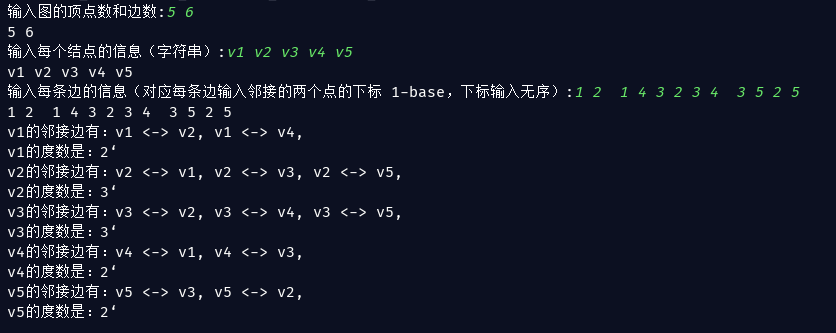
\includegraphics[width=0.8\textwidth,natwidth=700,natheight=470]{1.PNG}
        \caption{链表形式存储二叉树的基本操作}
      \end{figure}



\subsection{项目2.1}
大致思想 :线索二叉树,不递归,不用辅助栈,不用三叉。若结点的左儿子为空,让结点的左儿子指向该结点的前驱,右儿子为空,指向该结点的前驱后继。递归遍历一遍各个结点,构建二叉树的前序,中序线索。
\subsubsection{实验步骤}
\begin{enumerate}
\item 构造函数:复杂度O(1),建立根节点。
\item 析构二叉树:复杂度O(n), n为二叉树结点个数。       ***用辅助队列queue,层序遍历树的过程中,取出队首元素,删除队首元素的之前,将它的两个不是线索的非空儿子入队,再取出队首元素,直到队列为空为止。
\item 建立树CreateTree(string s):复杂度O(n), n为二叉树结点个数。与上述建立普通二叉树同理,只是构建新儿子时,要将其父亲结点的线索域置为LINK。
\item 建立前序线索树:复杂度O(n), n为二叉树结点个数。***preOrder\_threading(Node * p,Node *\& pre)前序递归建立线索。左儿子空,左儿子为p的前驱pre,若pre不空,且pre右儿子空,建立好pre的后继.更新pre.递归左右儿子建立线索,注意是真儿子LINK才能递归,否则,根据线索进入其前驱,前驱再访问到它,进入死循环。
\item 遍历前序线索二叉树:复杂度O(n), n为二叉树结点个数。***主调函数中,visit完当前结点,更新当前结点为当前结点的后继; preOrder\_successor\_thread(Node *p)函数寻找当前结点的后继:前序遍历的后继,如果左儿子不为空,后继就为左儿子,左儿子空,后继是右儿子(可能是真儿子,也可能是线索化后的后继)、
\item 建立中序线索二叉树:复杂度O(n), n为二叉树结点个数。*** 同上,只把建立线索的模块和递归语句顺序调换。建立线索的模块需要做:已知 pre 和p 的关系: 即pre 的后继是p 和 p 的前驱是 pre ,根据这两个关系可以分别对 pre 和 p 建立线索
\item 遍历中序线索二叉树:复杂度O(n$log_2 n$), n为二叉树结点个数。***中序遍历。第一个visit的是最左下的结点,所以先找到它,进入循环visit它,再找它的后继。找后继:x的右子是线索指针,正好指向x的中序后继,是真儿子,后继就是右儿子最左下的点。
\end{enumerate}
\subsubsection{必要代码}
\lstinputlisting[language=C++]{code/code2/main.cpp}
\subsubsection{实验结果}如图2
	\begin{figure}[!bthp]
	\centering
    
		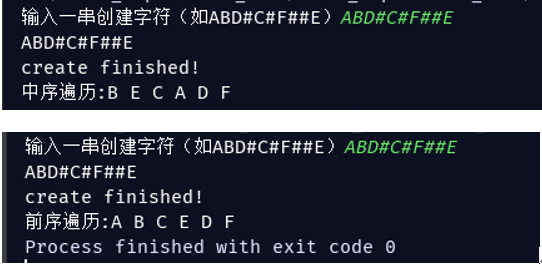
\includegraphics[width=0.8\textwidth,natwidth=700,natheight=200]{2.1.PNG}
        \caption{线索二叉树的前序后序遍历}
      \end{figure}


\subsection{项目2.2}
大致思想 :三叉树,相比较普通二叉树,多了一个指向父亲节点的指针。遍历的过程中,可以利用parent回到原结点。
三叉链表的深度遍历,依然可以递归来完成。整个过程和二叉链表版本没有任何区别。但是非递归版本   不用辅助栈也不用递归。如下实现。
\subsubsection{实验步骤}
\begin{enumerate}
\item 构造函数:复杂度O(1),建立根节点。
\item 析构二叉树:复杂度O(n), n为二叉树结点个数。      ***同理,用辅助队列queue,层序遍历树的过程中,取出队首元素,删除队首元素的之前,将它的两个儿子入队,再取出队首元素,直到队列为空为止。
\item 建立树CreateTree(string s):复杂度O(n), n为二叉树结点个数。与上述建立普通二叉树同理,只是构建结点新儿子时,要将其儿子结点的parent域置为该结点。
\item 三叉前序遍历:复杂度O(n$log_2 n$), n为二叉树结点个数。***重点分析找后继的函数preOrder\_Successor(Node* p):p如果有儿子,后继一定是直系儿子,p 为叶子结点 后继为父亲结点的右儿子。若右儿子为空 或者 p就为父亲的右儿子,后继为换方向后的那个转折点的右儿子。
\item 三叉中序遍历:复杂度O(n$log_2 n$), n为二叉树结点个数。***中序遍历。第一个visit的是最左下的结点,所以先找到它,进入循环visit它,再找它的后继。找后继:inOrder\_Successor(Node *x).如果x有右结点,则所求定是其x的右子树中最左下的点,否则就是x的祖先结点中的某个(遇到转折点)。
\item 三叉后序遍历:复杂度O(n$log_2 n$), n为二叉树结点个数。***第一个访问的结点:find\_first\_node\_postOrder(root)注意,第一个访问的就不一定是最左下的点:p的左子不空,就为左子,右子不空,就为右子,否则就为自己。postOrder\_Successor(Node *p)找后继:根节点的后继为空;p 为父亲的右儿子,后继即p的父亲; p为父亲的左儿子, 说明其父亲 和父亲的右儿子都还没访问,先访问父亲的右儿子,如果右儿子为空,接下只能访问父亲,父亲的右儿子不为空,用find\_first\_node\_postOrder(cur)找右儿子的第一个访问的结点。
\end{enumerate}
\subsubsection{必要代码}
\lstinputlisting[language=C++]{code/code2.0/main.cpp}
\subsubsection{实验结果}如图3
	\begin{figure}[!bthp]
	\centering
       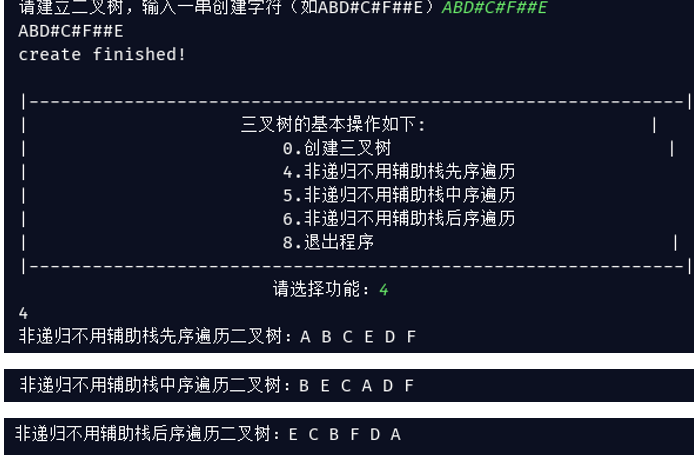
\includegraphics[width=0.8\textwidth,natwidth=610,natheight=300]{2.2.PNG}
        \caption{三叉树的前中后序遍历}
      \end{figure}



\subsection{项目3}
大致思想 :有序存储树BST,结点结构体中有key值,左儿子,右儿子,父亲指针,通过比较结点key值大小插入结点来创建BST树,建立结点内部的联系。
有序代表能像链表或是栈等结构,增/删/改/查 某个结点;AVL除了 插入 和 删除,其他继承BST。BST和AVL查找结点和树高的关系测试:向BST和AVL上插入同样的随机生成的1000000个结点,观察他们的插入时间和生成的树高,再寻找同样的随机生成的100 000个结点,比较查找总时间。
\subsubsection{实验步骤}
\begin{enumerate}
\item BST构造函数:复杂度O(1)
\item 析构二叉树:复杂度O(n), n为二叉树结点个数。      ***BFS遍历一遍二叉树,利用辅助队列,逐个释放所有结点
\item 创建BST  Create\_BST( int n) : 复杂度O(nh), n为二叉树结点个数, h为二叉树的高度 。  *** 通过插入创建,与节点数量有关,每插入一次,最坏的情况是查到最底部。
\item 递归插入:复杂度O(h), h为二叉树的高度      *** 一直递归,直到找到合适的位置插入为止。
\item 非递归插入:复杂度O(h), h为二叉树的高度      *** 一直循环比较结点key值大小,直到找到合适的位置插入为止。
\item 递归和非递归search 某个值(查找最小值,最大值同理):复杂度O(h), h为二叉树的高度  ***最坏的情况为从树根一直找到底部
\item  找后继:复杂度O(h), h为二叉树的高度      *** node 的右子树不为空,则 node 的后继就是它的右子树中最左下的点(即关键字值最小的结点);右节点为空,只要还没到根节点,或者node 还是p 的右儿子,左中右,说明它的父亲已经被访问,还要顺藤向上
\item  找前驱:复杂度O(h), h为二叉树的高度      ***  与找后继镜像对称
\item  删除结点:复杂度O(h), h为二叉树的高度 , 其中种树:Transplant(Node *T, Node *u,Node *v) 复杂度O(1)   ***二叉查找树的删除操作是相对复杂一点,它要按 3 种情况来处理:删除(Deletion):从T中删除节点z,三种情况:1) z没有孩子, 简单将其父节点的指向 z的指针替换为NIL;
2) z只有1个孩子 将z的这个孩子提升为z的父亲的孩子,取代z的位置;
3) z有俩孩子 先找z的中序后继y(必然在z的右子树), y取代z的位置, z中右子树剩下的部分成为y的新右子树,z的左
   树变成y的新左树. (第三种情况比较复杂,取决于y是不是z的右孩),//其中1的情况可以合并到2 (因为可以用NULL取代z 的位置)
\item 修改结点:复杂度O(h), h为二叉树的高度;  ****先删除这个结点,再插入新结点,这两个操作都是O(h);
\item  前序中序遍历上述三叉链表已经分析。
\item AVL除了 插入 和 删除,其他继承BST,这里只分析 插入和删除的复杂度,旋转操作的复杂度都是常数
\item  AVL递归插入结点:复杂度O(h), h为二叉树的高度      ***只在为 v的插入位置寻找新结点产生O(h)的复杂度
\item  AVL非递归插入结点:复杂度O(h), h为二叉树的高度      ***为插入结点寻找合适父亲t,产生O(h)的复杂度,插入后修复函数AVL\_Insert\_Fixup(NewNode->parent),从传入结点开始,往上修复,直到遇到根节点为止,
\item  AVL删除结点:复杂度O(h), h为二叉树的高度      *** 只在为 查找要删除的结点v时产生O(h)的复杂度,修复函数AVL\_Delete\_Fixup(Node *p)//修正不平衡的树复杂度O(1)
\item  主函数中,测试BST和AVL查找结点和树高的关系测试:复杂度O($n^2$+$n^2$*h), n为二叉树结点个数,h为二叉树的高度  ***测试的外部循环O(n);内部产生随机数:需要一个n规模的循环生成有效随机数,一个n规模的循环将下标赋值。内部插入,查询结点:并且n规模的循环插入,寻找结点.且插入,查询操作复杂度O(h)
\end{enumerate}
\subsubsection{必要代码}
\lstinputlisting[language=C++]{code/code3/main.cpp }
\lstinputlisting[language=C++]{code/code3/BST.h}
\lstinputlisting[language=C++]{code/code3/AVL.h}
\subsubsection{实验结果}如图4 和5 和6
	\begin{figure}[!bthp]
	\centering
        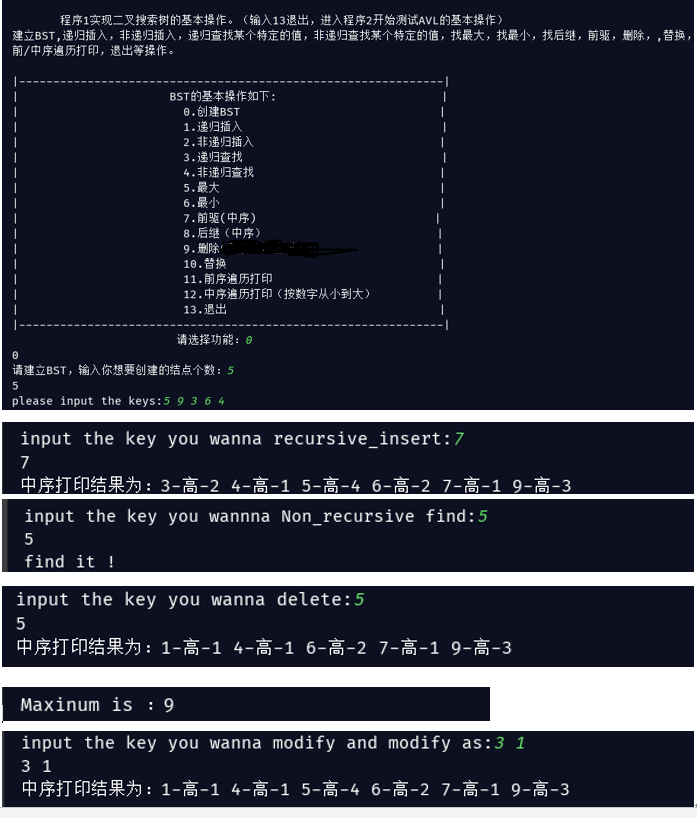
\includegraphics[width=0.8\textwidth,natwidth=610,natheight=450]{3.1.PNG}
        \caption{BST的基本操作}
      \end{figure}
\begin{figure}[!bthp]
	\centering
         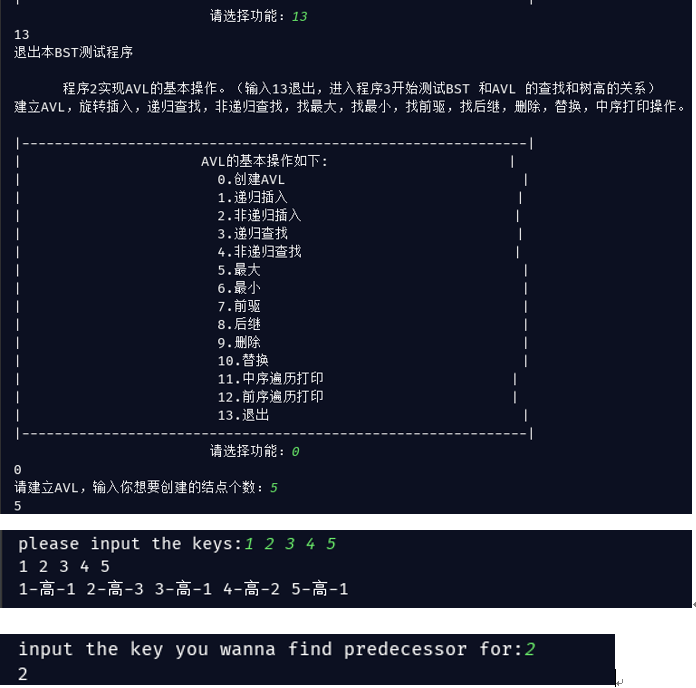
\includegraphics[width=0.8\textwidth,natwidth=610,natheight=400]{3.2.PNG}
        \caption{AVL的基本操作}
      \end{figure}

\begin{figure}[!bthp]
	\centering
         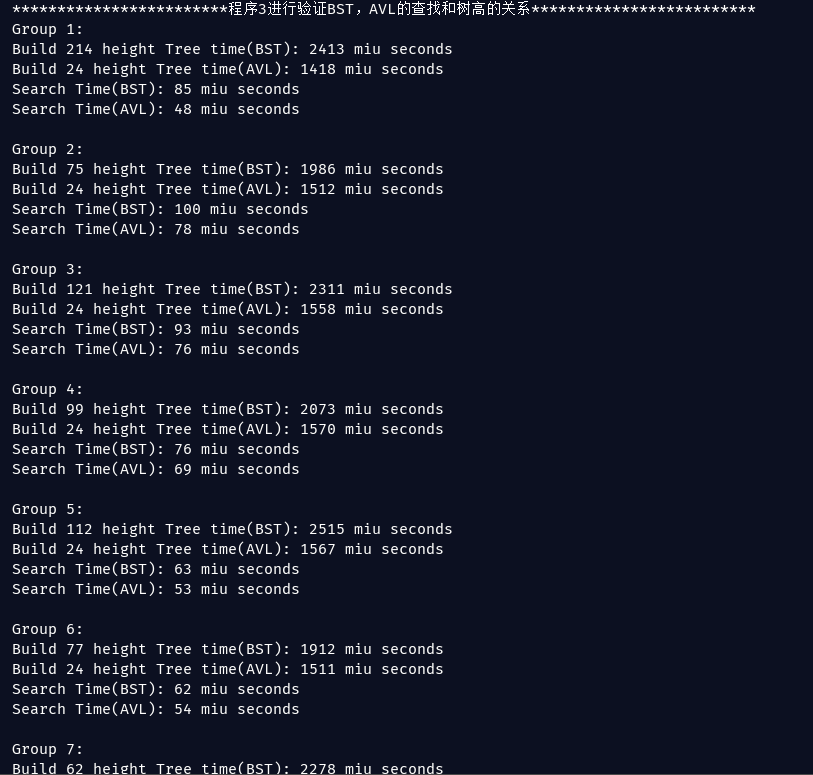
\includegraphics[width=0.8\textwidth,natwidth=610,natheight=450]{3.3.PNG}
        \caption{BST和AVL查找结点和树高的关系测试}
      \end{figure}


\subsection{项目4}
大致思想 :每个结点是一个结构体,里面有char类型的结点代号,权值,string类型的编码code,左右儿子指针。利用最小堆,每次取堆顶元素,构建huffman树的新结点,再将新结点入堆(新结点的权值等于原来结点权值之和)。直到堆中元素取完为止.
\subsubsection{实验步骤}
\begin{enumerate}
\item 创建哈夫曼最小堆::复杂度O(n), n为待编码的节点个数     ***一个n规模的循环,为新结点开辟空间和填入信息
\item 堆化操作(递归):复杂度O(logn) = O(h) ,n为堆数组有效长度,h堆树高    ***递归逐步向下调整
\item 建堆1-based:复杂度O(h) ,h堆树高     *** 自底向上将数组调整为一个最小堆,从第一个非叶子结点开始查它和它儿子的关系
\item 拿出二叉堆中最小元素O(h):复杂度O(h) ,h堆树高  ***虽然每次取得最小值的复杂度O(1),但是还要调整堆的结构
\item 最小堆插入:复杂度O(h) ,h堆树高  ***每次插入还要调整堆的结构
\item 堆排序:复杂度O(nh) ,h堆树高, n为堆数组有效长度  ***堆排序(将数组中的元素从小到大排列),同时逐渐瓦解二叉堆的二叉树结构;循环调整n此,每次将最后一个元素和第一个元素交换,再最小化堆。
\item 建哈夫曼树:复杂度O(hlogn),h堆树高, n哈夫曼树结点个数     ***外层循环,直到堆数组元素取完为止,内部,每次取两个结点,再插入一个结点。
\item 建立编码:复杂度O(n), n为哈夫曼二叉树的结点个数     ***(前序)遍历过程中编码,每到一个非叶子结点,,从左边过来就在string类型编码
中+"0",从右边过来就在string类型编码中+"1",遍历完成,编码也完成。
\item 明文转编码:复杂度O(nm), n为哈夫曼叶子结点个数,m输入字符串长度。    ***遍历字符串的每个字符,对于每个字符,在堆数组中寻找对应的结点代号的编码,输出
\item 解码:复杂度O(nm), n为哈夫曼叶子结点个数,m输入字符串长度。    ***逐个读入编码,遍历堆数组,若没找到,读入的编码数增加一个;直到编码串结束为止

\end{enumerate}
\subsubsection{必要代码}
\lstinputlisting[language=C++]{code/code4/main.cpp}
\lstinputlisting[language=C++]{code/code4/MinHeap.h}
\lstinputlisting[language=C++]{code/code4/Huffman.h}
\subsubsection{实验结果}如图 7
	\begin{figure}[!bthp]
	\centering
        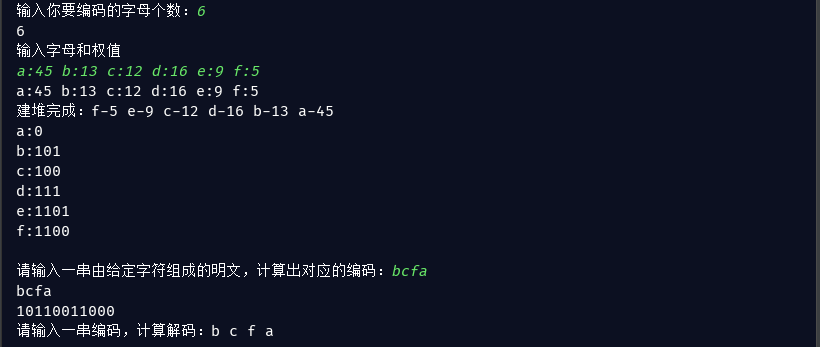
\includegraphics[width=0.6\linewidth]{4.PNG}
        \caption{哈夫曼解码和编码}
      \end{figure}


\subsection{项目5}
由项目3 一并完成,详情请见项目3


\section{实验总结}
\begin{enumerate}
\item 本次实验测得BST与AVL建树和查找的效率:对于相同的结点,AVL数建立用时较短且树高稳定,而BST树高波动较大,这就导致在后续查找过程中,查找时间波动大,且查找时间比AVL长。
\item 最小堆建立二叉树比较方便
\item 存在问题:BST和AVL非递归 更新树高未完成;线索二叉树后序建立线索未完成。
\end{enumerate}

\end{document}
